\chapter{Kata Containers}
\label{chapter:katacontainers}

The emergence of container technology provides a lightweight operating-system-level virtual hosting environment. Its emergence profoundly changes the development and deployment paradigms of multi-tier distributed services. However, due to the incomplete implementation of system resource isolation mechanisms in the Linux kernel, security concerns still exist for a multi-tenancy container cloud service \cite{Gao2017}. Securing cloud and edge computing services from malicious actors is crucial for companies and MNOs to secure users, services, and data confidentiality and privacy. Kata Containers offers an up-and-coming solution to enhance security with the lightweight isolation layer and compatible integration to the current container orchestration environment. This chapter describes the Kata Container's architecture, components, and features compared to the current container architecture.

\section{Kata Containers}

Service latency is often the most important criteria for selecting a container execution environment. Slow response times can impair the usability of an edge computing infrastructure. Higher service latencies also result in higher average resource utilization and, therefore, in lower achievable throughput \cite{EverartsdeVelp2020}. Meanwhile, securing container runtime is a crucial task in MEC to run multiple instances in the same edge securely. Therefore, multiple solutions have been developed to provide more robust workload isolation using hardware virtualization technology as a second layer of defense. One of the most prominent approaches includes wrapping the container inside a micro VM during run time. Micro VM is a lightweight version of traditional VM with reduced overhead stemming from OS, libraries, dedicated resources, and applications in full VM \cite{Flauzac2020}. Micro VM includes a separate mini kernel to create an isolated environment for the container \cite{Kumar2020}. This dedicated kernel of micro VM provides isolation of network, I/O, and memory and can utilize hardware-enforced isolation with virtualization extensions. In this Thesis, we will focus on Kata Containers as a secure container runtime. Kata Containers perform like containers but provide the workload isolation and security advantages of VMs. Thus, combining the benefits of containers and VMs. \cite{KataContainers}

Kata Containers is open source and licensed under the Apache 2.0 license. An Architecture Committee drives the development. Contributors elect the committee's members, who oversee architectural decisions, such as standardization, and resolve technical disagreements between project maintainers. Currently, five members from Apple, Intel, Ant Financial, and Red Hat comprise the committee. \cite{KataContainers}\cite{KataContainersGovernance}

\section{Architecture}

Kata Containers originates from Intel's Clear Containers \cite{ClearContainers} and Hyper runV \cite{runV} in December 2017. The architecture aims to build extremely lightweight VMs that perform like containers but provide the workload isolation and security advantages of adding a virtual machine layer \cite{Randazzo2019}. The design philosophy behind Kata Containers is to integrate seamlessly to the current industry standard of publishing applications as containers. Kata Containers requires no changes to the containers themselves, as the only modification is required on the container orchestrator and the container runtime. Kata Containers integrates into the process of launching and managing the container in the host platform. The main problem Kata Containers is solving is balancing the trade-off between security and speed. In this Thesis environment, Kata Containers is deployed within Kubernetes. Figure \ref{fig:KataContainersArchitecture} demonstrates the latest architecture defined version 2.0. This architecture comprises six elements: Kubernetes, container manager, shim, hypervisor, agent, and VM.

Kubernetes is the container orchestrator and resource manager for automating deployment. Runtime and shim integrate to container manager such as containerd. The runtime uses a hypervisor to provide isolation by creating a lightweight VM for each container and then running containerd inside the VM. The Kata container project has introduced a daemon that runs inside the kata-agent virtual machine for managing the containers. This agent uses libcontainer to manage the lifecycle of a container. Kata uses a highly optimized guest kernel to boot the virtual machine, which offers minimal memory usage and fast boot time. This guest kernel provides a better isolated environment for containers than the traditional security mechanisms of process isolation in containers. \cite{Kumar2020}

Kata Containers, which the OpenStack Foundation stewards, supports industry standards and has been designed along with the OCI specifications, thus it supports all the OCI runtime operations \cite{Kumar2020}. As any OCI compliant runtime, the Kata Containers works seamlessly with the Kubernetes Container Runtime Interface (CRI)\cite{CRI}, as well as legacy virtualization technologies, through the container manager such as containerd or CRI-O implementation \cite{Randazzo2019}.

\begin{figure}[ht]
  \begin{center}
    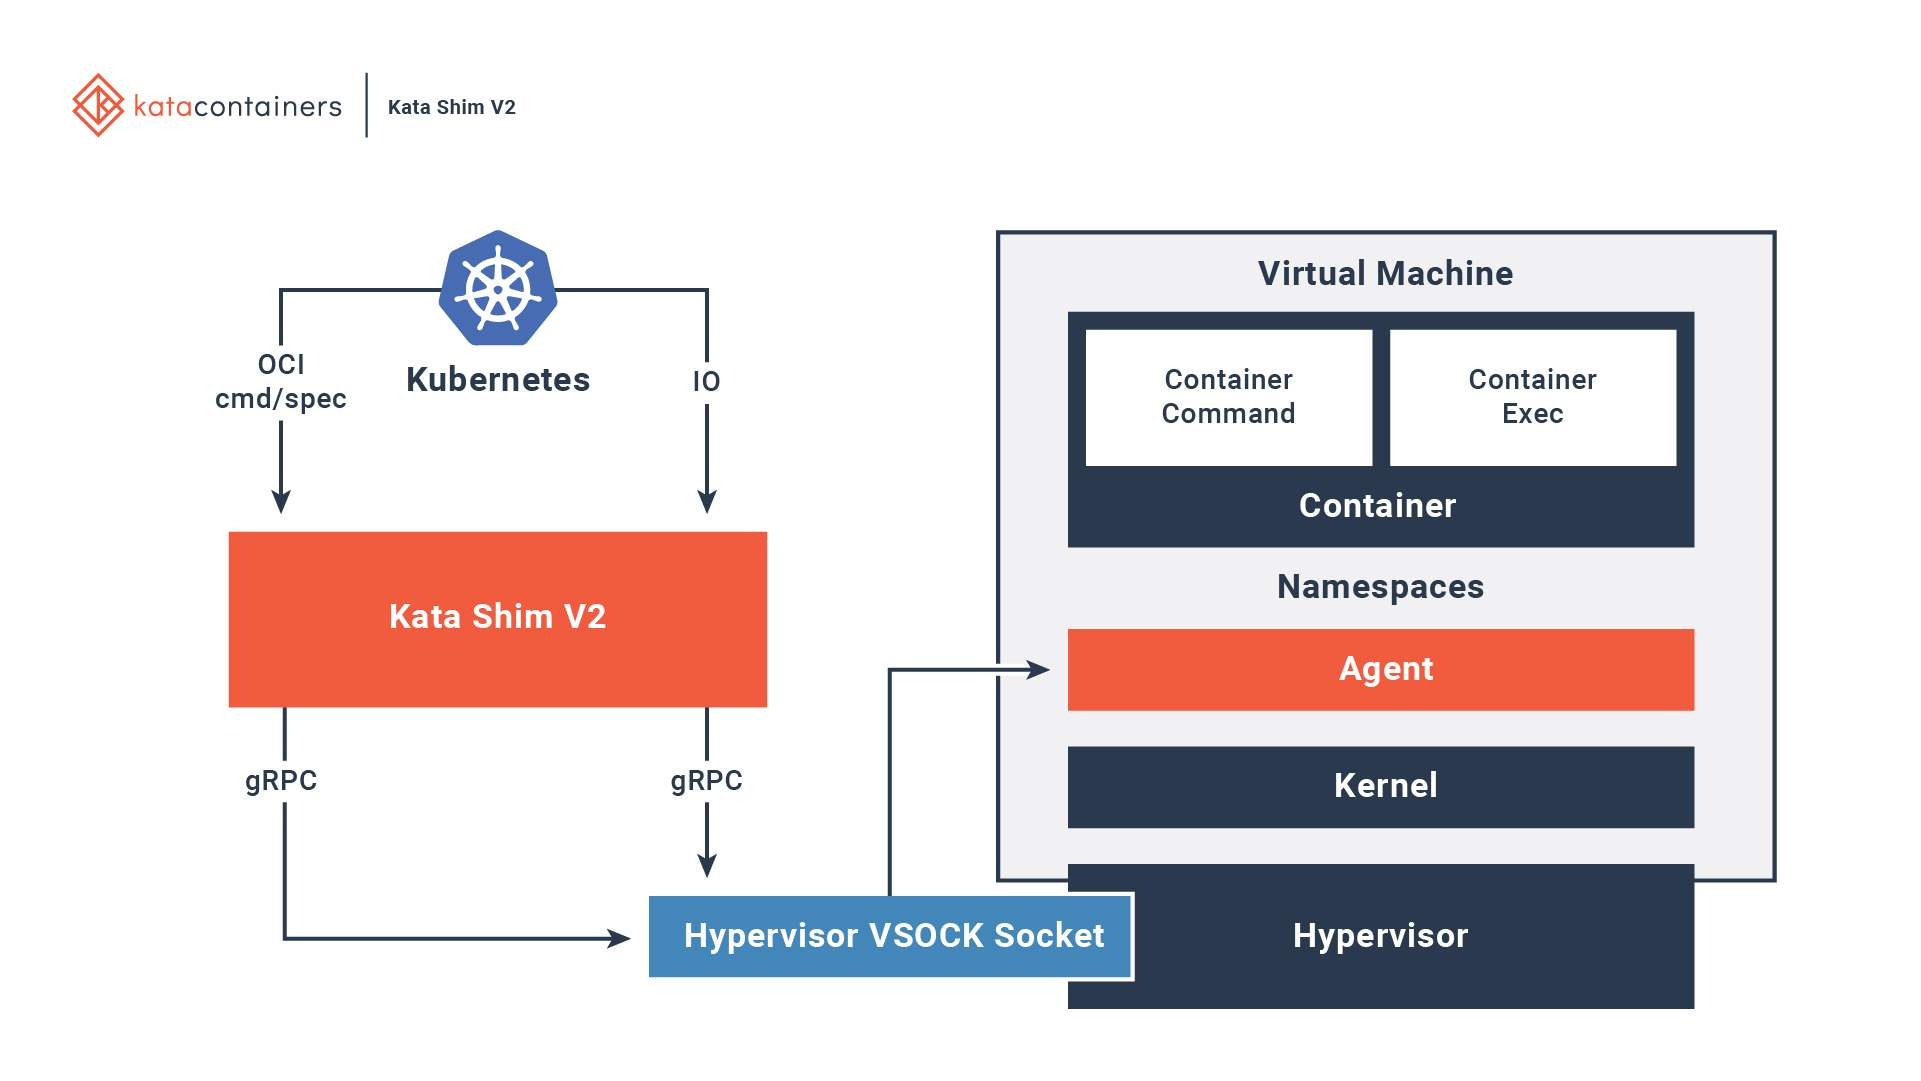
\includegraphics[width=13.5cm]{images/KataContainersArchitecture.jpg}
    \caption{Kata Containers 2.0 architecture \cite{KataContainers}}
    \label{fig:KataContainersArchitecture}
  \end{center}
\end{figure}

\begin{figure}[ht]
  \begin{center}
    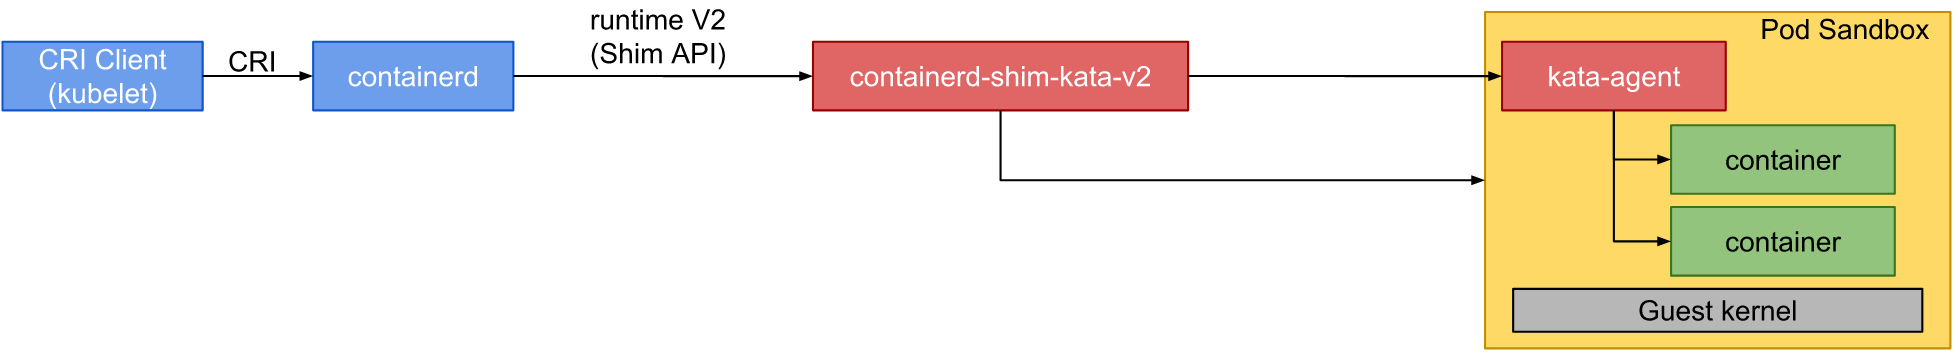
\includegraphics[width=13.5cm]{images/KataContainersComponents.png}
    \caption{Kata Containers 2.0 components \cite{KataContainersArchitecture}}
    \label{fig:KataContainersComponents}
  \end{center}
\end{figure}

\subsection{Kubernetes}

Kubernetes is an open-source container orchestration tool developed by Google. Kubernetes automates deployment, scaling, and management of containerized applications \cite{Kubernetes}. Kubernetes monitors the state of containers in the system, and the containers can be automatically re-created in a case of failure \cite{Toimela2017}. Kubernetes offers flexible configuration, and it can be installed inside a VM or on bare-metal. 

Kubernetes launches each container as a pod. Pods are the atomic unit on the Kubernetes platform. A single node can include multiple pods inside it and ties each pod into it within the creation of the pod. Like most distributed computing platforms, a Kubernetes cluster consists of at least one master node and multiple compute nodes. Worker nodes run a node agent Kubelet, which communicates with the master node acting as the workload manager. The master node can also act as a worker node, for example, in a single node cluster. Kubernetes uses a container networking interface (CNI)\cite{CNI} component to provide an overlay network for the pods. Each node includes a CNI.

Each compute node runs a container runtime engine, such as Docker or containerd, along with an agent communicating with the master node. The runtime can be selected on a pod level; thus, a single node can consist of workloads with various runtimes. This flexibility of concurrent runtimes comes in handy whenever non-confidential but highly performance-centric applications need to be deployed in a node within more security-oriented applications.

\subsection{Containerd}

As the Docker project grew, it extracted the container runtime engine into a new project containerd\cite{containerd}. Container runtime engine manages containers inside Kubernetes, including functionality for executing containers, handling low-level storage, and managing image transfers. Containerd is an open-source implementation of the Kubernetes CRI to enable usage of OCI compatible runtimes. It is an industry-standard container runtime with an emphasis on simplicity, portability, and robustness. It is available as a daemon for Linux and Windows, which can manage the complete container lifecycle of its host system. The flexibility of containerd allows Kubernetes to register and use various OCI-compliant runtimes, such as Kata Containers, as container runtime for running pods. Containerd supports multiple means to download images, including trust and image verification. Containerd also manages container process lifecycles, low-level storage, and resource isolation as required by the CRI. \cite{containerdGithub}

\subsection{Kata Shim V2}

The primary deliverable of the Kata Containers project is a CRI-friendly shim. In the latest version merges the shim, proxy, and runtime into one component. The shim launches Kata-Agent, which launches the container itself. Kata runtime is an OCI compatible container runtime and can handle commands specified by the OCI runtime specification. These commands include invoking the hypervisor for creating a lightweight and fast VM for each container in a pod and launching the Kata Containers instances \cite{Randazzo2019}. The shim enables daemonless containers, allowing the runtime to exit after the container has been launched and then becomes the container's parent. Kata-Agent continues to communicate with other Kata Containers components over RPC \cite{KataContainersArchitecture}. \cite{Crosby}

\subsection{gRPC and ttRPC}

gRPC is a high-performance Remote Procedure Call framework that can run in any environment. It connects services in and across data centers with pluggable support for load balancing, tracing, health checking, and authentication. This protocol allows the runtime to send container management commands to the agent. The protocol also to handles the I/O streams such as stdout, stderr, and stdin between the containers.
gRPC manages the container engine, which is containerd in this Thesis. Using gRPC via VSOCK interface avoids using previously maintained proxy component as the VSOCK interface can multiplex all gRPC requests \cite{Randazzo2019}. \cite{gRPC}\cite{KataContainersArchitecture}

However, gRPC requires a lot of memory overhead for importing packages and at runtime. While this is great for many services with low-density requirements, this can be a problem when running a large number of services on a single machine or a machine with a small amount of memory. ttRPC also offers harnessed security by limiting attack surface and improved observability via metrics about the runtime itself, the VMM, as well as the guest kernel. Kata Shim V2 offers the support for ttRPC protocol to communicate with the agent. \cite{ttRPC}

\subsection{Hypervisor}

VM of Kata Containers instance is launched by VMM, which consists of Virtual Machine Manager and a hypervisor. Kata Containers currently supports four different VMMs: ACRN hypervisor, Cloud Hypervisor, QEMU, and Firecracker. All these VMMs are open-source projects.

ACRN, a reference hypervisor, is built to meet the needs of embedded IoT development. It is developed with low overhead, fast boot-up, and configurations to support various devices and deployment scenarios. ACRN is a type 1 reference hypervisor stack that runs on bare-metal hardware, addressing the gap between data center hypervisors and hard partitioning hypervisors. \cite{ACRN}

Cloud Hypervisor is a VMM that runs on top of the Kernel-based Virtual Machine (KVM). The project focuses on exclusively running modern cloud workloads on top of a limited set of hardware architectures and platforms. Customers inside a cloud provider usually run cloud workloads, and most I/O operations are handled by performant para-virtualized devices, such as Virtio. \cite{CloudHypervisor}

QEMU is a generic machine, userspace emulator, and virtualizer. QEMU is capable of emulating a complete machine in software without any need for hardware virtualization support. It can also integrate with the Xen and KVM hypervisors to provide emulated hardware while allowing the hypervisor to manage the CPU. Kata Containers uses a special version of QEMU name qemu-lite to improve boot time and reduce memory footprint with features such as machine accelerators, kernel same-page merging, hot plug devices, and Fast Template \cite{Randazzo2019}. \cite{QEMUGithub}\cite{QEMU}

Machine accelerators are architecture-specific for improving performance. One of these enables direct access storage, allowing sharing the host rootfs in read-only mode to a persistent memory device to the VMs. Kernel same-page merging is a KVM feature that allows sharing identical memory pages amongst different VMs. This sharing deduplicates memory to maximize container density on a host. Hot-plug devices allow VMs to start with minimum resources for faster boot time and a tiny memory footprint. The hypervisor allocates the VM more resources as soon as requested by hot-plugging devices on the fly. Fast Template is a pool of pre-configured lightweight VMs ready to deploy quickly. \cite{Randazzo2019}

Firecracker is community driven VMM, backed and originally developed by AWS. Firecracker uses KVM to launch workload in lightweight micro virtual machines. Of Amazon's cloud products, Firecracker is deployed at least in AWS Lambda and Fargate. Firecracker currently supports Intel CPUs, with AMD and Arm support in developer preview. \cite{AWS}\cite{FirecrackerDesign}\cite{Debab2021}

\subsection{Agent}

Agent, also known as Kata-Agent, resides inside the Kubernetes pod in the computing node, and its main task is to spawn the container process. The agent sets up the environment for managing containers and processes running within those containers. The agent process runs as a daemon inside the virtual machine. This agent runs a ttRPC or gRPC server in the guest using a Virtio serial or VSOCK interface, which the VMM exposes as a socket file on the host. \cite{KataContainersArchitecture}

\subsection{Container}

Kata Containers architecture isolates a container by wrapping it inside a dedicated kernel. This extra layer provides isolation of the network by minimizing container escapes of a malicious actor. I/O and memory can utilize hardware-enforced isolation with virtualization VT extensions. Wrapping the container inside a micro VM adds an overhead to performance, which is discussed more in Chapter \ref{chapter:evaluation}. \cite{KataContainers}

Kata Containers is OCI compliant; thus, the same standard shared by Docker containers guarantees compatibility. For now, only Linux operating systems and container images are supported in host and guest.

\section{Features}

The architecture and components of Kata Containers allow a different approach to hosting containers in the environment compared to Docker runtime. The most crucial feature of Kata Containers is the extra layer of isolation provided by the micro VM. Due to this isolation layer, some changes are needed to the network layer to allow OCI compatible networking for the container runtime engine, further discussed in this section.

\subsection{Isolation and resource allocation}

Kubernetes environment deploys application containers inside a pod. Upon creating a pod, it requests resources, which most commonly are CPU, memory, and huge pages, defined in the configurations. The allocated resources are reserved for the application running. Traditionally the resources allocated are a slice from the resource described in Figure \ref{fig:KataContainersStack}. Kata Containers environment virtualizes the hardware for the guest kernel.

Kata Containers, a second layer of isolation, is created on top of traditional namespace containers. The hardware virtualization interface is the basis of this additional layer. Kata Containers launches a lightweight virtual machine and uses the guest's Linux kernel to create a container workload. In Kubernetes and the Kata implementation, the sandbox is carried out at the pod level. A virtual machine such as KVM creates the sandbox for workload isolation \cite{KataContainersVirtualization}. Because KVM is a hypervisor emulating complete hardware and hosts another Linux kernel inside, it is considered even harder to escape this environment resulting in harnessed security \cite{Eder2016}.

The additional layer of isolation allows untrusted workloads to be run in the same system without compromising other containers' security. Container escapes, as mentioned in Chapter \ref{section:security}, have been a severe threat to a system using traditional container isolation mechanisms such as namespaces, cgroups, and seccomp.

\begin{figure}[ht]
  \begin{center}
    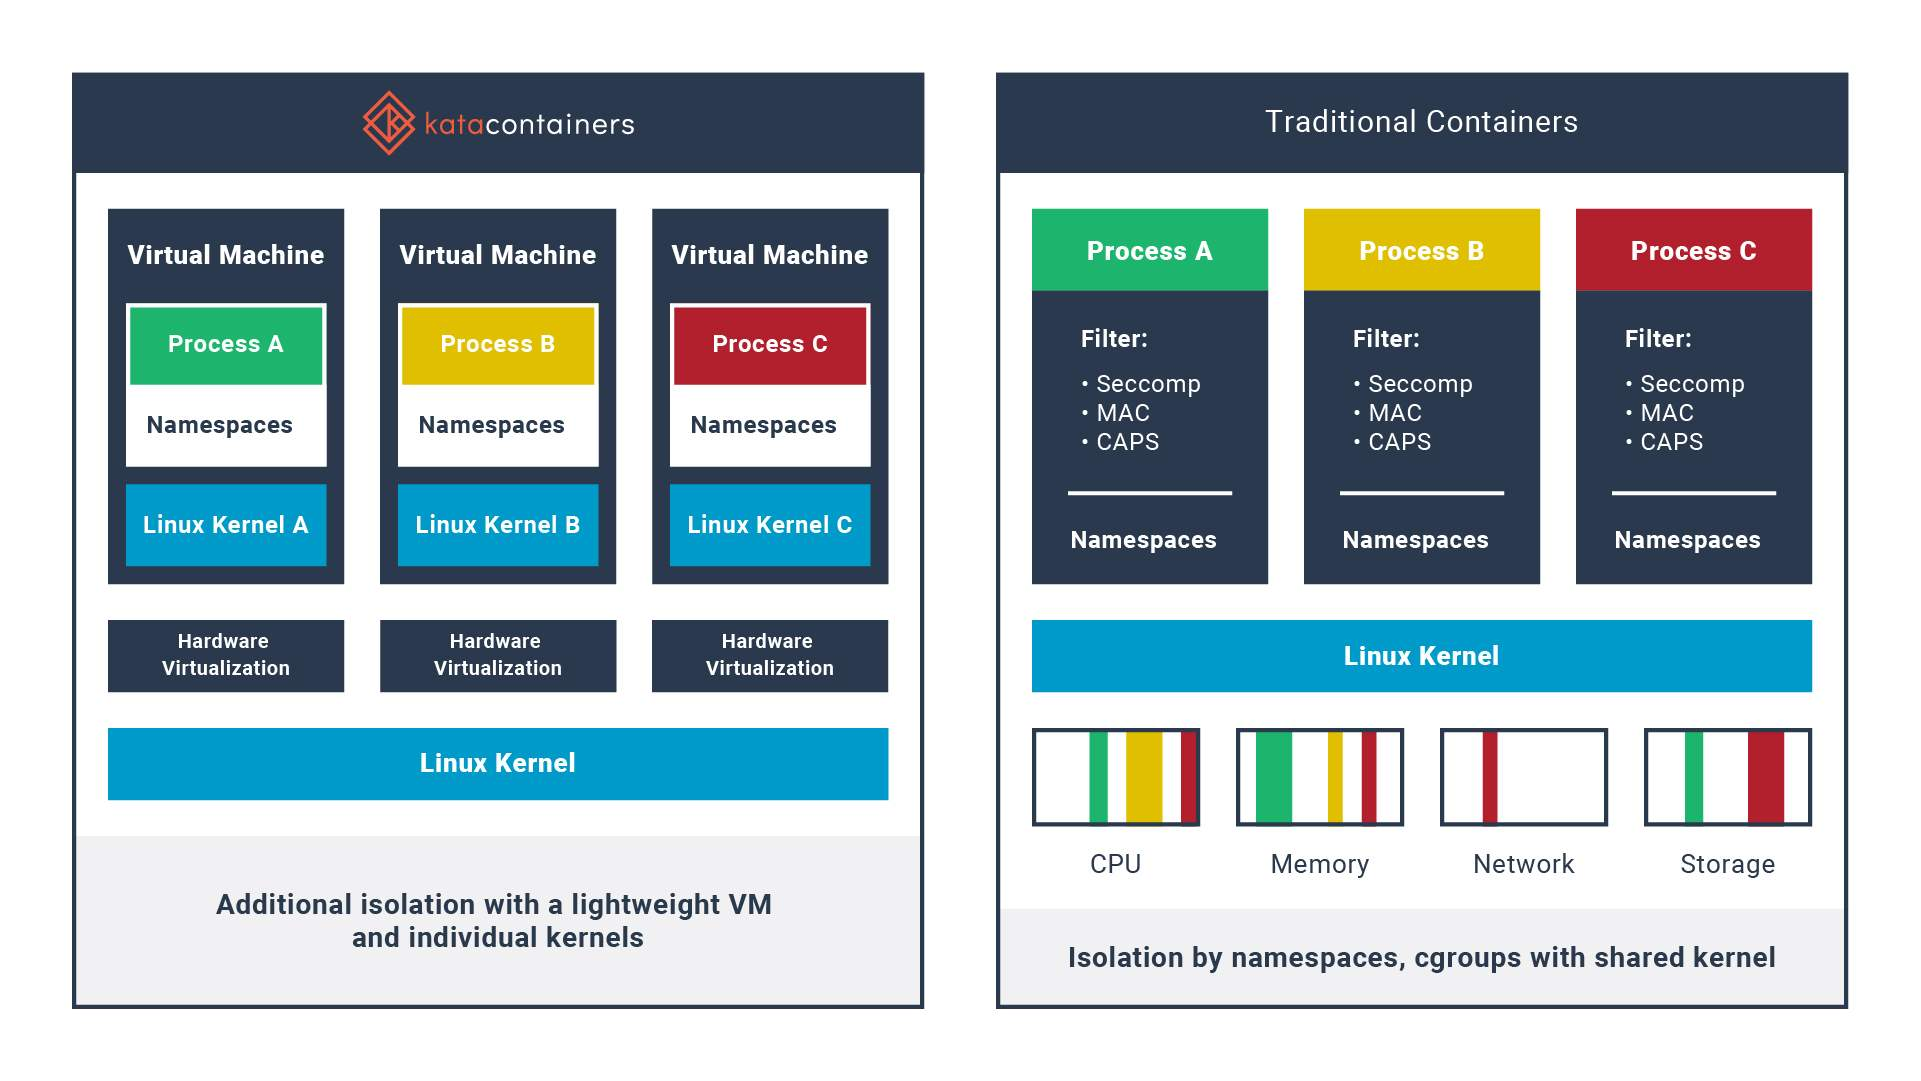
\includegraphics[width=13.5cm]{images/KataContainersStack.jpg}
    \caption{Kata Containers and traditional container stack \cite{KataContainers}}
    \label{fig:KataContainersStack}
  \end{center}
\end{figure} 

\subsection{Networking}

Traditionally container engines, such as Docker, add one end of a virtual ethernet pair into the container networking namespace. The other end of the pair is added to the host networking namespace. However, many VMMs cannot handle virtual ethernet interfaces. Typically, TAP interfaces are created for VM connectivity. As described in Figure \ref{fig:KataContainersNetwork} Kata runtime overcomes the incompatibility between typical container engine's expectations and virtual machines by connecting virtual ethernet interfaces to kernel virtual network device TAP using Traffic Control. TAP works on data link layer carrying ethernet frames and is often used to create a user-space network bridge. \cite{KataContainersArchitecture}

Kata Containers supports both container network models (CNM) adopted by Docker and CNI adopted by Kubernetes and Podman. Both models provide the freedom of selection for a specific type of container networking, join one or more networks, and use multiple network drivers concurrently \cite{Randazzo2019}. Kata supports both IPv4 and IPv6 networks.

\begin{figure}[ht]
  \begin{center}
    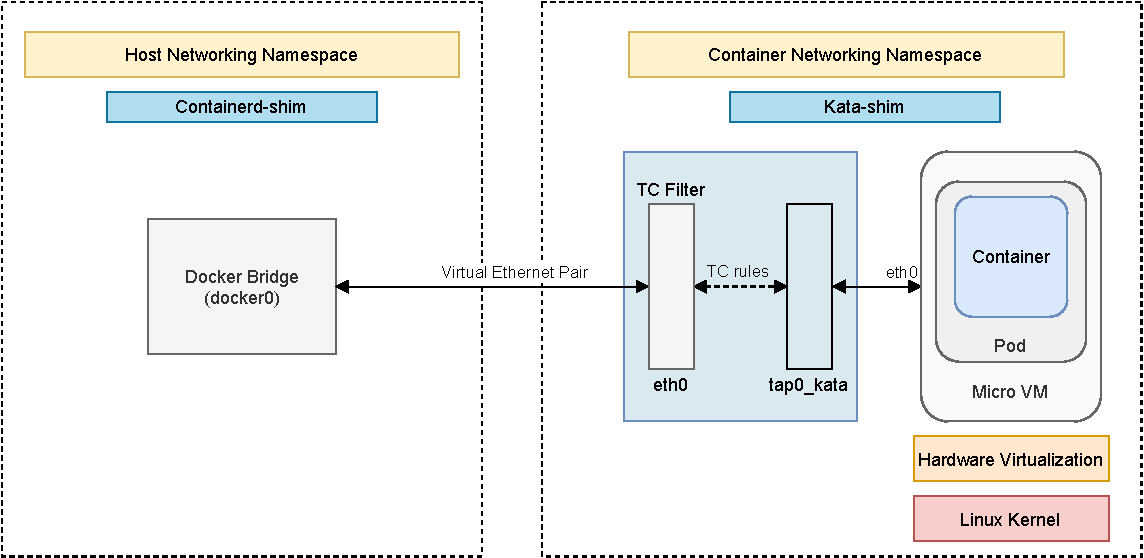
\includegraphics[width=13.5cm]{images/KataContainersNetwork.pdf}
    \caption{Kata Containers network overview \cite{KataContainersArchitecture}}
    \label{fig:KataContainersNetwork}
  \end{center}
\end{figure}

\subsection{Storage}

Kata Containers can manage the storage both at the file system level and at the block level. At the file system level, virtualized environment shares container workloads through virtio-fs. This shared file system permits VMs to access a directory tree on the host. Kata Containers uses virtio-fs to share container volumes, secrets, config-maps, configuration files, and the container rootfs on the host with the guest. Virtio-fs provides significant performance and POSIX compliance improvements compared to 9pfs, supported in Kata Containers. Virtio-fs was started at Red Hat and developed in the Linux, QEMU, FUSE, and Kata Containers open source communities. \cite{virtio-fs-Kata}\cite{virtio-fs}

Kata Containers can hot-plug and remove block devices, a data storage device that supports reading and optionally writing data in fixed-size blocks, sectors, or clusters. This support for hot-plugging makes it possible to add new block devices for containers started after launching the VM without a reboot. Hot-plugging adds flexibility and improves the uptime of services. Regardless of general support for hot-plugging and various file systems, its exact compatibility might vary depending on the VMM and hypervisor. \cite{KataContainersArchitecture}\cite{KataContainersVirtualization}

\section{Summary}

Kata Containers offers a potential solution for lightweight workload isolation compatible with current Kubernetes and container environments, harnessing the benefits of container orchestration. Kata Container's architecture includes several components differing from the current defacto standard. Regardless of this difference, the basic functionalities such as block and filesystem storages and Docker-like networking interface are offered to support OCI standards.